\documentclass[10pt,twocolumn]{extarticle}
\usepackage[a4paper,margin=1.5cm,columnsep=0.7cm]{geometry}
\usepackage{amsmath,amssymb}
\usepackage{graphicx}
\usepackage{enumitem}
\usepackage{booktabs}
\usepackage{array}
\usepackage{tabularx}
\usepackage[T1]{fontenc}

\setlength{\parindent}{0pt}
\setlength{\parskip}{4pt}
\renewcommand{\arraystretch}{1.15}

\newenvironment{qoptions}{\begin{itemize}[leftmargin=1.8em,itemsep=2pt,topsep=2pt,label={}]}{\end{itemize}}
\newcommand{\opt}[2]{\item[({#1})] {#2}}

\newcommand{\sectionhdr}[1]{\par\vspace{4pt}\noindent\textbf{\large #1}\par\vspace{2pt}}
\newcommand{\subsectionhdr}[1]{\par\vspace{3pt}\noindent\textbf{#1}\par\vspace{2pt}}

\pagestyle{empty}

\begin{document}
\twocolumn[
\begin{center}
{\LARGE\bfseries JEE (Main+Advanced) Score-II --- Test 01 (21 Mar 2021)}
\end{center}
\vspace{6pt}
]

\sectionhdr{PAPER-1}

\sectionhdr{PART-1: PHYSICS}
\subsectionhdr{Section-I (i): Multiple Choice (one or more correct)}

\textbf{1.} In a radioactive decay reaction $A \xrightarrow{\lambda} B \xrightarrow{2\lambda} C$. Select correct alternative(s) at the instant the number of particles of B is maximum:
\begin{qoptions}
\opt{A}{Activity of A is equal to activity of B.}
\opt{B}{No. of atoms of A is 2 times of B.}
\opt{C}{Activity of A is more than activity of B.}
\opt{D}{Activity of B is maximum.}
\end{qoptions}

\textbf{2.} The two slits of double slit experiment were moved symmetrically apart with small relative velocity $v$ and the distance between screen and mid-point of slits is fixed and equal to $D$. Consider a point P on the screen at a distance $x$ from central maxima then ($x \ll D$):
\begin{qoptions}
\opt{A}{Rate of change of number of fringes between central maxima and point P changes with respect to time is $\dfrac{xv}{\lambda D}$.}
\opt{B}{Number of fringes contained between central maxima and point P increases with time.}
\opt{C}{Fringe width decreases as time passes.}
\opt{D}{Maximas are moving closer to each other.}
\end{qoptions}

\textbf{3.} A simple bar magnet hangs from a string as in figure. A uniform magnetic field $\vec{B}$ directed horizontally to the right is then established. Which of the pictures in figure does not show the equilibrium orientation of the bar magnet?

\begin{center}
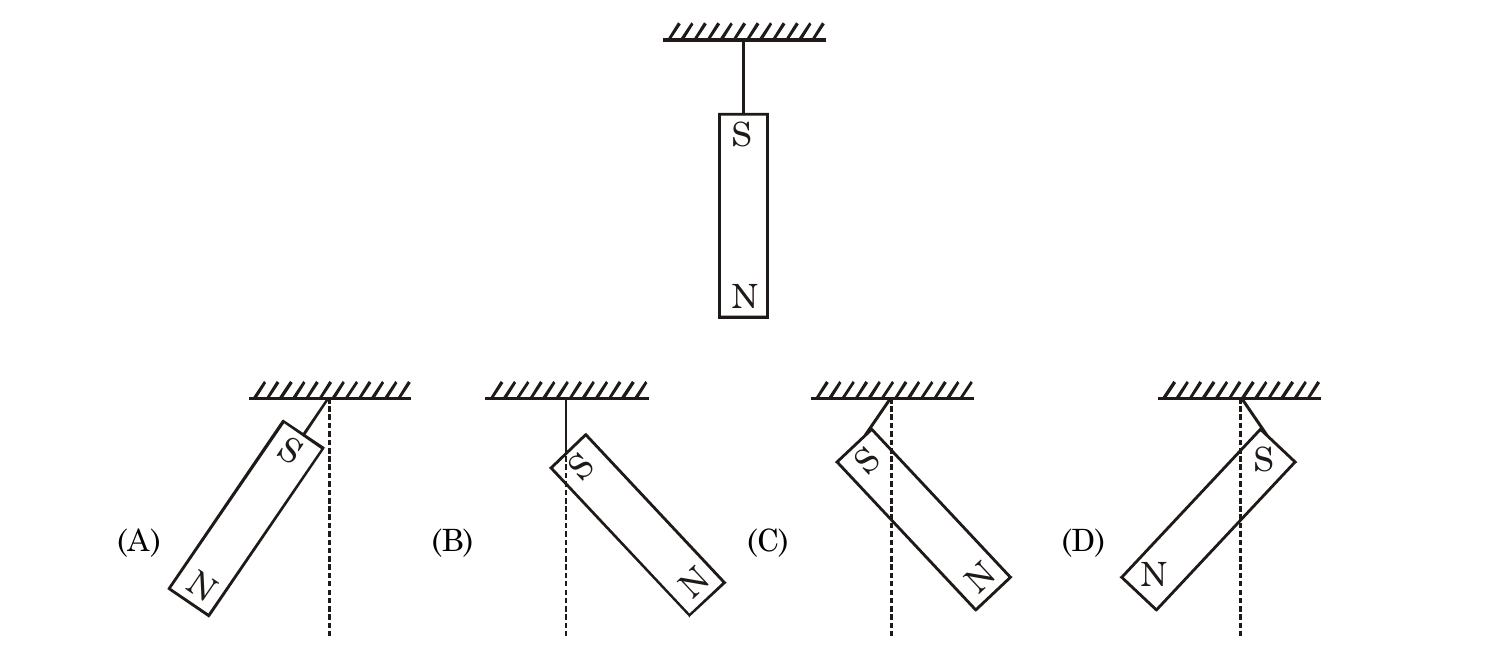
\includegraphics[width=0.95\linewidth]{Score-II - Test 01 (21 Mar 2021)-img/p1-phys-q3.png}
\end{center}

\textbf{4.} A particle constrained to move along $x$-axis given a velocity $u$ along the positive $x$-axis. The acceleration $a$ of the particle varies as $a = -bx$, where $b$ is a positive constant and $x$ is the $x$ co-ordinate of the position of the particle. Then select the correct alternative(s):
\begin{qoptions}
\opt{A}{The maximum displacement of the particle from the starting point is $\dfrac{u}{\sqrt{b}}$.}
\opt{B}{The particle will oscillate about the origin.}
\opt{C}{Speed is maximum at the origin.}
\opt{D}{Angular frequency of oscillation is $b$.}
\end{qoptions}

\textbf{5.} Lower end of a capillary tube of radius $10^{-3}$ m is dipped vertically into a liquid. Surface tension of liquid is 0.5 N/m and specific gravity of liquid is 5. Contact angle between liquid and material of capillary tube is $120^{\circ}$. Choose the correct options (use $g = 10$ m/s$^2$):
\begin{qoptions}
\opt{A}{Maximum possible depression of liquid column in the capillary tube is 1 cm.}
\opt{B}{Maximum possible depression of mercury column in the capillary tube is 2 cm.}
\opt{C}{If the length of the capillary tube dipped inside mercury is half of the maximum possible depression of mercury column in the capillary tube, angle made of the mercury surface at the end of the capillary tube with the vertical, is $\cos^{-1}\left(-\dfrac14\right)$.}
\opt{D}{If the length of the capillary tube dipped inside mercury is one third of the maximum possible depression of mercury column in the capillary tube, angle made by the mercury surface at the end of the capillary tube with the vertical, is $\cos^{-1}\left(-\dfrac16\right)$.}
\end{qoptions}

\textbf{6.} A car moves towards a hill with speed $v_C$. It blows a horn of frequency $f$ which is heard by an observer following the car with speed $v_0$. The speed of sound in air is $v$.
\begin{qoptions}
\opt{A}{The frequency of sound reaching the hill is $\left(\dfrac{v}{v-v_C}\right)f$.}
\opt{B}{The wavelength of sound reaching the hill is $\dfrac{v-v_c}{f}$.}
\opt{C}{The wavelength of sound of horn directly reaching the observer is $\dfrac{v+v_c}{f}$.}
\opt{D}{The beat frequency observed by the observer is $\dfrac{2v_C(v+v_0)f}{v^2-v_C^2}$.}
\end{qoptions}

\subsectionhdr{Section-I (ii): Matching / Paragraph (single correct)}

\textit{Paragraph for Questions 7 and 8:} In physics laboratory a student is trying to calculate the focal length of a convex lens. He measures the distance between screen and a light source lined up on the optical bench to be 120 cm. When he shifts the lens along the axis of optical bench, sharp image of source is obtained at two lens positions. He also measures the ratio of these two magnifications to be $1:9$.

\textbf{7.} The focal length of the convex lens measured by student is
\begin{qoptions}
\opt{A}{22.5 cm}
\opt{B}{30 cm}
\opt{C}{45 cm}
\opt{D}{none of these}
\end{qoptions}

\textbf{8.} Which image, as seen by student is brighter?
\begin{qoptions}
\opt{A}{smaller}
\opt{B}{bigger}
\opt{C}{both are equally bright}
\opt{D}{can not be judged}
\end{qoptions}

\textit{Paragraph for Questions 9 and 10:} A block of mass $3M$ connected to a massless rod of length $L$ lies at rest on a fixed frictionless table. A second block of mass $M$ impinges on the system with speed $v_0$, strikes the opposite end of the rod at a right angle and sticks to it.

\begin{center}
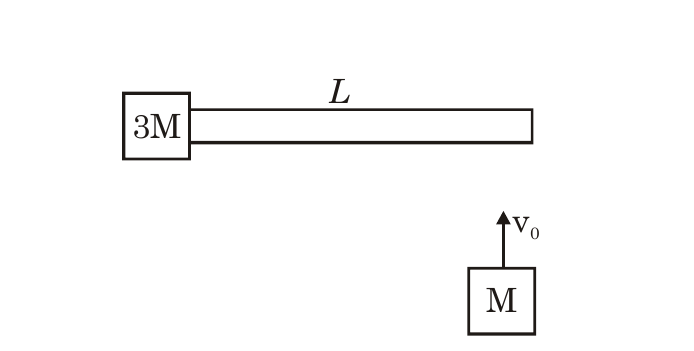
\includegraphics[width=0.7\linewidth]{Score-II - Test 01 (21 Mar 2021)-img/p1-phys-q9-10.png}
\end{center}

\textbf{9.} Angular velocity of new system about its COM is
\begin{qoptions}
\opt{A}{$\dfrac{v_0}{L}$}
\opt{B}{$\dfrac{v_0}{2L}$}
\opt{C}{$\dfrac{3v_0}{4L}$}
\opt{D}{$\dfrac{4v_0}{3L}$}
\end{qoptions}

\textbf{10.} Initial velocity of $3M$ after collision is
\begin{qoptions}
\opt{A}{$\dfrac{3v_0}{4}$}
\opt{B}{zero}
\opt{C}{$\dfrac{v_0}{2}$}
\opt{D}{$\dfrac{v_0}{4}$}
\end{qoptions}

\subsectionhdr{Section-II: Numerical Value}

\textbf{1.} A human body excretes certain material by a law similar to radioactivity. The body excretes half the amount injected in 24 h. Find the time in which activity falls to $3\,\mu$Ci (in hours) if a person is injected technetium ($t_{1/2}=6$h) and its activity just after the injection is $6\,\mu$Ci.

\textbf{2.} Two conducting spheres of radius $R$ are placed at a large distance from each other. They are connected by a coil of inductance $L$, as shown in the figure. Neglect the resistance of the coil. The sphere A is given a charge $Q$ and the switch $S$ is closed at time $t=0$. Time after charge on B is $\dfrac{Q}{2}$ is $\dfrac{\pi}{a}\sqrt{\dfrac{LR}{k}}$. Then value of $a$ is:

\begin{center}

\includegraphics[width=0.85\linewidth]{Score-II - Test 01 (21 Mar 2021)-img/p1-phys-num-q2.png}
\end{center}

\textbf{3.} A charged capacitor ($C_1 = 3\,\mu$F) is getting discharged in the circuit shown. When the current $I$ was observed to be 2.5 A, switch $S$ was opened. Determine the amount of heat (in $\mu$J) that will be liberated in the circuit after $S$ is opened.

\begin{center}
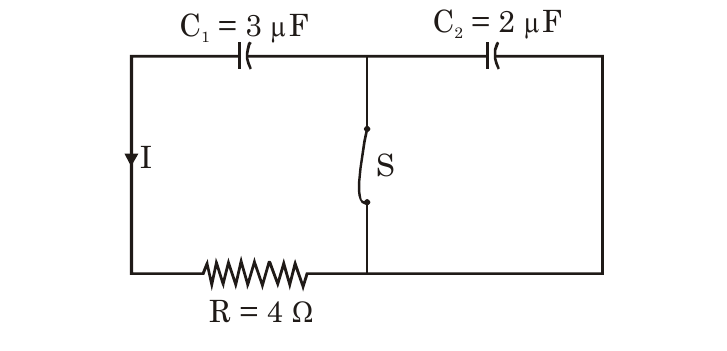
\includegraphics[width=0.8\linewidth]{Score-II - Test 01 (21 Mar 2021)-img/p1-phys-num-q3.png}
\end{center}

\textbf{4.} Three short electric dipoles, each of dipole moment $P$, are placed at the vertices of an equilateral triangle of side length $L$. Each dipole has its moment oriented parallel to the opposite side of the triangle as shown in the figure. The electric field strength at the centroid of the triangle is $a\dfrac{KP}{L^3}$. Then value of $a$ is:

\begin{center}
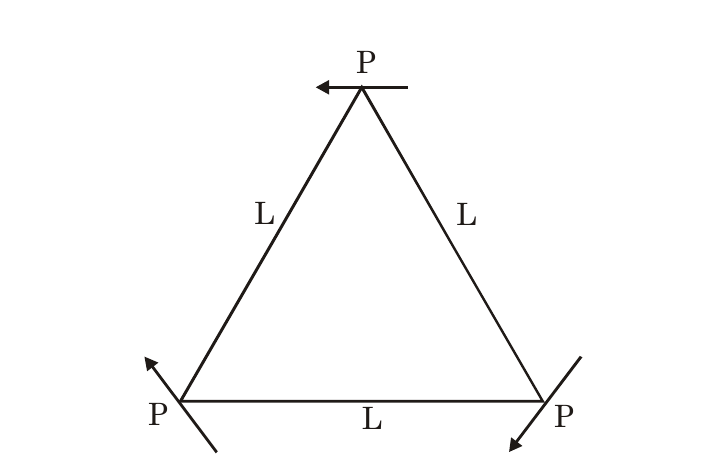
\includegraphics[width=0.6\linewidth]{Score-II - Test 01 (21 Mar 2021)-img/p1-phys-num-q4.png}
\end{center}

\textbf{5.} In a vernier calliper, there are 10 divisions on the vernier scale and 1 cm on main scale is divided in 10 parts. While measuring a length, the zero of the vernier scale lies just ahead of 1.8 cm mark and 4th division of vernier scale coincides with a main scale division. The value of length (in cm) is

\textbf{6.} 1 g ice at $-40^{\circ}$C is placed in a container having 1 g water at $20^{\circ}$C. Find equilibrium temperature (in $^{\circ}$C).
Water equivalent of container $=3$ gm; Latent heat of fusion of ice $=80$ cal/gm; Specific heat capacity of water $=1$ cal/gm$^{\circ}$C; Specific heat capacity of ice $=0.5$ cal/g$^{\circ}$C.

\textbf{7.} A point-like mass moves horizontally between two walls on a frictionless surfaces with initial kinetic energy $E$. With every collision with the walls, the mass loses 50\% of its kinetic energy to thermal energy. How many collisions with the walls are necessary before the speed of the mass is reduced by a factor of 8 (means it becomes $\tfrac18$th of initial speed)?

\textbf{8.} The velocity of liquid ($v$) in steady flow at a location through cylindrical pipe is given by $v = v_0\left(1-\dfrac{r^2}{R^2}\right)$, where $r$ is the radial distance of that location from the axis of the pipe and $R$ is the inner radius of pipe. If $R=10$ cm, volume rate of flow through the pipe is $\pi/2 \times 10^{-2}$ m$^3$s$^{-1}$ and the coefficient of viscosity of the liquid is 0.75 N sm$^{-2}$, find the magnitude of the viscous force per unit area, in Nm$^{-2}$ at $r=4$ cm.

\sectionhdr{PART-2: CHEMISTRY}
\subsectionhdr{Section-I (i): Multiple Choice (one or more correct)}

\textbf{1.} Which of the following statements is/are INCORRECT:
\begin{qoptions}
\opt{A}{All spectral lines belonging to Balmer series in hydrogen spectrum lie in visible region.}
\opt{B}{If a light of frequency $\nu$ falls on a metal surface having work function $h\nu_0$, photoelectric effect will take place only if $\nu \le \nu_0$.}
\opt{C}{The number of photoelectrons ejected from a metal surface in photoelectric effect depends upon the frequency of incident radiations.}
\opt{D}{The series limit wavelength of Balmer series of H-atom is $\dfrac4R$, where R is Rydberg's constant.}
\end{qoptions}

\textbf{2.} Which one of the following statements is/are incorrect?
\begin{qoptions}
\opt{A}{The principal ore of aluminium; bauxite usually contains silica, ironoxide and titanium oxide as impurity}
\opt{B}{Limonite, magnesite and haematite are ores of iron}
\opt{C}{The Anode mud in electrolytic refining of silver contains Cu and Au.}
\opt{D}{During calcinations at high temperatures sulphide ores of some metal like Cu, Pb, Hg are reduced directly into metal.}
\end{qoptions}

\textbf{3.} Incorrectly matched amongst the following is/are:

\begin{center}
\begin{tabular}{@{}p{3.0cm}p{4.9cm}@{}}
\toprule
\textbf{Column-I} & \textbf{Column-II} \\
\midrule
(A) 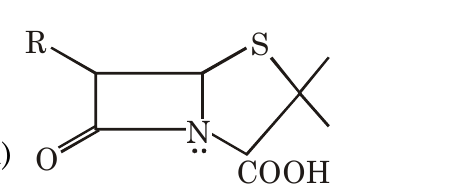
\includegraphics[width=2.6cm]{Score-II - Test 01 (21 Mar 2021)-img/p1-chem-q3-A.png} \newline Bicyclic amide &
Resonance is restricted due to non-planarity \\[4pt]
(B) 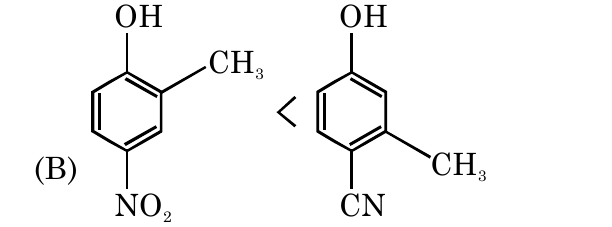
\includegraphics[width=2.6cm]{Score-II - Test 01 (21 Mar 2021)-img/p1-chem-q3-B.png} \newline Acidic Strength &
Reason being $-$CN is a better $-$M group than $-$NO$_2$ \\[4pt]
(C) 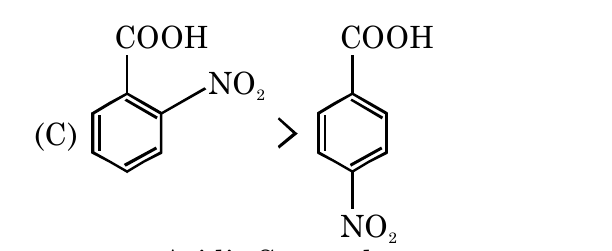
\includegraphics[width=2.6cm]{Score-II - Test 01 (21 Mar 2021)-img/p1-chem-q3-C.png} \newline Acidic Strength &
Reason being $-$M effect of $-$NO$_2$ group at ortho is more than that at para. \\[4pt]
(D) 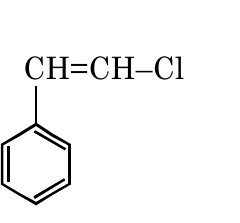
\includegraphics[width=1.4cm]{Score-II - Test 01 (21 Mar 2021)-img/p1-chem-q3-D.png} \newline is an o/p directing group &
$-$CH=CH$-$Cl is an activating group \\
\bottomrule
\end{tabular}
\end{center}

\textbf{4.} Which of the following are correct?
\begin{qoptions}
\opt{A}{$K_{sp}$ of Fe(OH)$_3$ in aqueous solution is $3.8\times10^{-38}$ at 298K. The concentration of Fe$^{3+}$ will increase when [H$^+$] ion concentration decreases}
\opt{B}{In a mixture of NH$_4$Cl and NH$_4$OH in water, a further amount of NH$_4$Cl is added. The pH of the mixture will decreases.}
\opt{C}{An aqueous solution of each of the following salts (NH$_4$I, Cr(NO$_3$)$_3\cdot$9H$_2$O, KCN) will be basic, basic, acidic respectively.}
\opt{D}{From separate solutions of four sodium salts NaW, NaX, NaY and NaZ had pH 7.0, 9.0, 10.0 and 11.0 respectively, when each solution was 0.1M, the strongest acid is HW}
\end{qoptions}

\textbf{5.} Aqueous solution of boric acid is treated with salicylic acid. Which of the following statements are incorrect for the product formed in above reaction.
\begin{qoptions}
\opt{A}{No product will be formed because both are acids.}
\opt{B}{Product is 4-coordinated complex and optically resolvable.}
\opt{C}{Product is 4-coordinated complex and optically non-resolvable.}
\opt{D}{There are two newly formed five membered rings.}
\end{qoptions}

\textbf{6.} Correctly matched among the following is/are:

\begin{center}
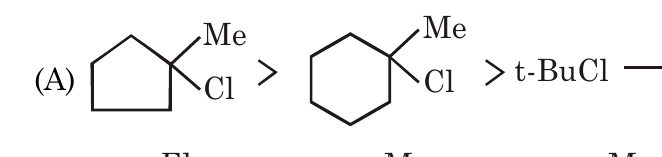
\includegraphics[width=0.95\linewidth]{Score-II - Test 01 (21 Mar 2021)-img/p1-chem-q6-A.png}
\end{center}
\vspace{-2pt}
(A) Relative Solvolysis Rate order shown above.

(B) $\text{Me-}\overset{\displaystyle\text{El}}{\underset{\displaystyle\text{Et}}{\text{C}}}\text{-Cl} \;>\; \text{Me-}\overset{\displaystyle\text{Me}}{\underset{\displaystyle\text{Et}}{\text{C}}}\text{-Cl} \;>\; \text{Me-}\overset{\displaystyle\text{Me}}{\underset{\displaystyle\text{Me}}{\text{C}}}\text{-Cl}$ --- Rate of hydrolysis in 80\% aq. ethanol

(C) $\text{CH}_3\text{-Br} > (\text{CH}_3)_2\text{CH-CH}_2\text{-Br} > (\text{CH}_3)_3\text{CCH}_2\text{-Br}$ --- Relative rate of reaction with ethanol

(D) $\text{R}_2\text{N-CH}_2\text{X} > \text{R-CO-CH}_2\text{X} > \text{CH}_2\text{=CH-CH}_2\text{X}$ --- Order for rate of S$_N^{\,\prime}$ reaction

\subsectionhdr{Section-I (ii): Matching / Paragraph (single correct)}

\textit{Paragraph for Questions 7 and 8:} Dependence of rate constant of a reaction is given by Arrhenius equation $k = A\cdot e^{-E_a/RT}$ but originally it's derived from its differential equation.

\textbf{7.} Reactions A + B $\to$ C + D follows following rate law: rate $= k[A]^{+1/2}[B]^{1/2}$. Starting with initial conc. of one mole of A and B each, what is the time taken for amount of A to become 0.25 mole. Given $k = 2.31\times10^{-3}$ sec$^{-1}$.
\begin{qoptions}
\opt{A}{300 sec.}
\opt{B}{600 sec.}
\opt{C}{900 sec.}
\opt{D}{None of these}
\end{qoptions}

\textbf{8.} For a reaction, the dependence of rate constant (sec$^{-1}$) on temperature (K) is given as
\[\ln K = 10 - \frac{2500}{T} + 3\ln T\]
The activation energy of reaction is
\begin{qoptions}
\opt{A}{$2500+3T$}
\opt{B}{$2500\,R$}
\opt{C}{$(2500+3T)R$}
\opt{D}{$(2500-3\ln T)R$}
\end{qoptions}

\textit{Paragraph for Questions 9 and 10:} There are 4 glass bottles containing water solutions. These bottles are not labelled. Bottles 1, 2 and 3 contained colourless solutions, while Bottle 4 contained a coloured solution. Each bottle is having any solution among the following (each bottle is having different solution): copper (II) sulphate, sodium carbonates, lead nitrate, hydrochloric acid.

By mixing samples of the contents of the bottles in pairs, the following observations are made:
\begin{center}
\begin{tabular}{@{}ll@{}}
\toprule
Mixture & Observation \\
\midrule
Bottle 1 + Bottle 2 & White ppt. \\
Bottle 1 + Bottle 3 & White ppt. \\
Bottle 1 + Bottle 4 & White ppt. \\
Bottle 2 + Bottle 3 & Colourless gas evolved \\
Bottle 2 + Bottle 4 & No visible reaction \\
Bottle 3 + Bottle 4 & Blue ppt. \\
\bottomrule
\end{tabular}
\end{center}

\textbf{9.} Aqueous solution in bottle 4 is reacted with excess of KI and then Na$_2$S$_2$O$_3$ solution is added to it. Which of the following statement is incorrect.
\begin{qoptions}
\opt{A}{Evolved I$_2$ is reduced}
\opt{B}{S$_2$O$_3^{2-}$ is converted into SO$_4^{2-}$ in the above reaction}
\opt{C}{aqueous solution in bottle 4 is CuSO$_4$}
\opt{D}{Na$_2$S$_2$O$_3$ is oxidised}
\end{qoptions}

\textbf{10.} Chemical formula of white ppt. formed in observation (3) is:
\begin{qoptions}
\opt{A}{PbCl$_2$}
\opt{B}{PbCO$_3$}
\opt{C}{CuCO$_3$}
\opt{D}{PbSO$_4$}
\end{qoptions}

\subsectionhdr{Section-II: Numerical Value}

\textbf{1.} 'X' $\xrightarrow{\text{HONO}}$ N$_2$ + H$_2$O + 'Y' (Rubbing alcohol used in Hand Sanitizer). Find out mass \% of Nitrogen in compound 'X'.

\textbf{2.} How many compounds or ions can be oxidised by H$_2$O$_2$ among the following: (1) AsO$_3^{-3}$ (2) SO$_4^{-2}$ (3) Fe$_2$(SO$_4)_3$ (4) NH$_2$-NH$_2$ (5) H$_2$S (6) PbS (7) O$_3$ (8) SO$_3^{2-}$ (9) Cl$_2$

\textbf{3.} For the couple at 25$^{\circ}$C Ag$_{(s)} \mid$ AgCl$_{(s)} \mid$ Cl$^-_{(aq)} \Vert$ Ag$^+_{(aq)} \mid$ Ag$_{(s)}$ where $k_{sp}$(AgCl) $=10^{-10}$, $\dfrac{2.303RT}{F}=0.06$, $\sqrt{0.41}=0.64$.

If initially in a 10 litre container, 1 mole KCl and 2 mole AgNO$_3$ are taken along with sufficient amount of Ag and AgCl in it then find the moles of AgCl changed after long time.

\textbf{4.} Find out the sum of position of electrophile only in the major product obtained on aromatic Electrophilic substitution reaction. (Considering Locant w.r.t. the OH group)

\begin{center}
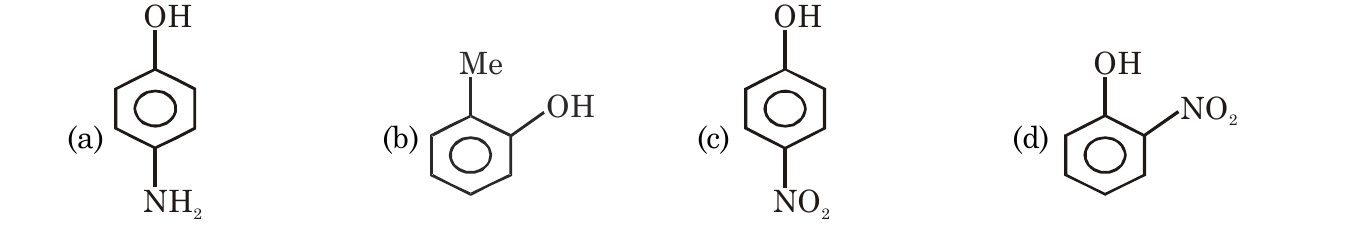
\includegraphics[width=0.95\linewidth]{Score-II - Test 01 (21 Mar 2021)-img/p1-chem-num-q4.png}
\end{center}

\textbf{5.} How many of the following compounds can be optically active?
(a) [Co(en)$_2$ClBr] \quad (b) [Co(en)(NH$_3)_2$Cl$_2$]$^+$ \quad (c) [Cr(NH$_3)_4$Cl$_2$]$^+$ \quad (d) [Co(NH$_3)_3$Cl$_3$] \quad (e) [Co(en)$_3$]$^{3+}$ \quad (f) [Ni(dmg)$_2$] \quad (g) [Pb(EDTA)]$^{2-}$ \quad (h) [Cr(ox)$_2$(NH$_3)_2$]$^-$ \quad (i) [Cr(gly)$_3$]

\textbf{6.} NaOH + HCl $\to$ NaCl + H$_2$O; \; Na$_2$CO$_3$ + HCl $\to$ NaHCO$_3$ + NaCl.

10 ml solution of 0.1 M NaOH and 0.1 M Na$_2$CO$_3$ is taken and 0.1 M HCl is added drop by drop. $pK_{a[\text{phenolphthalein}]} = 9.6$. For H$_2$CO$_3$, $pK_{a_1}=7$, $pK_{a_2}=11$.

pH of the solution when 25\% of the colour remains $= x$. Volume of HCl used in ml. for 25\% colour remaining $= y$. No. of unpaired electrons in coloured form $= z$ of indicator. Find $x+y+z$. Given: $10^{1.88}=75.85$, $\log 3 = 0.48$.

\textbf{7.} How many of the following is/are correct for Penicillin.
(a) It gives Black ppt with lead Acetate. [Lassaigne Test]
(b) It gives effervescence of CO$_2$ with NaHCO$_3$
(c) Presence of Lactum in its structure.
(d) It gives Red colour in Victor Mayer Test.
(e) It forms pungent smelling compound with CHCl$_3$ + NaOH
(f) It do not give violet colour with neutral FeCl$_3$
(g) It give +ve Mustard oil test.
(h) It give Prussian blue colour in Lassaigne Test
(i) 1 mol of Penicillin releases 1 mol of H$_2$(g) on treatment with Na.

\textbf{8.} In the given reaction, find out the molecular mass of 'X'.

\begin{center}
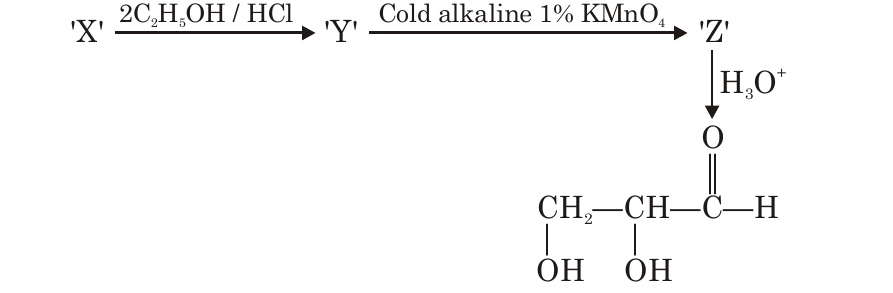
\includegraphics[width=0.95\linewidth]{Score-II - Test 01 (21 Mar 2021)-img/p1-chem-num-q8.png}
\end{center}

\sectionhdr{PART-3: MATHEMATICS}
\subsectionhdr{Section-I (i): Multiple Choice (one or more correct)}

\textbf{1.} Consider the following system of linear equations in x, y and z:
\[\begin{cases} px+qy+rz=0 \\ qx+ry+pz=0 \\ rx+py+qz=0 \end{cases} \;;\; p,q,r\in\mathbb{R}\]
If this system has non-trivial solution, then the system of equations may represent:
\begin{qoptions}
\opt{A}{planes meeting only at a single point}
\opt{B}{the line $x=y=z$}
\opt{C}{identical planes}
\opt{D}{whole 3d space}
\end{qoptions}

\textbf{2.} If a complex number $z$ satisfies the condition $\left|\log_{1/\sqrt3}\dfrac{|z|^2-|z|+1}{2+|z|}\right|<2$, then locus of $z$ may represent
\begin{qoptions}
\opt{A}{A circle having centre at origin and radius 1.}
\opt{B}{A ring between circles of radii 1 \& 5 with centre at origin.}
\opt{C}{Interior of a circle having radius $\dfrac13$ with centre as origin.}
\opt{D}{Exterior of a circle having radius 5.}
\end{qoptions}

\textbf{3.} From point A($-2,0$), tangents AB and AC are drawn to the parabola $y^2=8x$. A circle is drawn passing through the focus of the parabola and touching it at B and another circle is drawn passing through the focus of the parabola and touching it at C. Which of the following points with respect to $\triangle ABC$ lie on common chord of the two circles.
\begin{qoptions}
\opt{A}{incentre}
\opt{B}{centroid}
\opt{C}{circumcentre}
\opt{D}{orthocentre}
\end{qoptions}

\textbf{4.} In a triangle ABC, points D and E are taken on side BC such that BD $=$ DE $=$ EC. If $\angle ADE = \angle AED = \theta$, then:
\begin{qoptions}
\opt{A}{$\tan\theta = 3\tan B$}
\opt{B}{$3\tan\theta = \tan C$}
\opt{C}{$\dfrac{6\tan\theta}{\tan^2\theta-9}=\tan A$}
\opt{D}{$\angle B = \angle C$}
\end{qoptions}

\textbf{5.} Let $A = \begin{bmatrix}1&2&2\\2&1&2\\2&2&1\end{bmatrix}$, then
\begin{qoptions}
\opt{A}{$A^3-3A^2-9A-5I_3=0$}
\opt{B}{$A^{-1}=\dfrac15(A^2-3A-9I)$}
\opt{C}{$A^2$ is not invertible}
\opt{D}{$A^2$ is invertible}
\end{qoptions}

\textbf{6.} Which of the following is/are true?
\begin{qoptions}
\opt{A}{$\displaystyle\int_a^{\pi-a} x\,f(\sin x)\,dx = \dfrac{\pi}{2}\int_a^{\pi-a} f(\sin x)\,dx$}
\opt{B}{$\displaystyle\int_{-a}^{a} f^2(x)\,dx = 2\int_0^{a} f^2(x)\,dx$}
\opt{C}{$\displaystyle\int_0^{n\pi} f(\cos^2 x)\,dx = n\int_0^{\pi} f(\cos^2 x)\,dx,\; n\in\mathbb N$}
\opt{D}{$\displaystyle\int_0^{b-c} f(x+c)\,dx = \int_c^{b} f(x)\,dx$}
\end{qoptions}

\subsectionhdr{Section-I (ii): Matching / Paragraph (single correct)}

\textit{Paragraph for Questions 7 and 8:} Consider $f(x) = x^3(x-2)^2(x-1)$. On the basis of above information, answer the following questions:

\textbf{7.} If maxima of $f(x)$ occurs at $x_i$ then $\sum x_i^2$ is equal to
\begin{qoptions}
\opt{A}{$\dfrac94$}
\opt{B}{$\dfrac{25}{4}$}
\opt{C}{$\dfrac{40}{9}$}
\opt{D}{$\dfrac49$}
\end{qoptions}

\textbf{8.} Least value of $f(x)$ is
\begin{qoptions}
\opt{A}{$\dfrac19$}
\opt{B}{$\dfrac{4}{27}$}
\opt{C}{$-\dfrac{128}{729}$}
\opt{D}{0}
\end{qoptions}

\textit{Paragraph for Questions 9 and 10:} Let $f:\mathbb R\to\mathbb R$ be a function defined as
\[f(x)=\begin{cases}1-|x|, & |x|\le 1\\ 0, & |x|>1\end{cases}\]
\[g(x)=f(x-1)+f(x+1),\; \forall x\in\mathbb R.\]
Then

\textbf{9.} The function $g(x)$ is continuous for, $x\in$
\begin{qoptions}
\opt{A}{$\mathbb R-\{0,1,2,3,4\}$}
\opt{B}{$\mathbb R-\{-2,-1,0,1,2\}$}
\opt{C}{$\mathbb R$}
\opt{D}{None of these}
\end{qoptions}

\textbf{10.} The function $g(x)$ is differentiable for, $x\in$
\begin{qoptions}
\opt{A}{$\mathbb R$}
\opt{B}{$\mathbb R-\{-2,-1,0,1,2\}$}
\opt{C}{$\mathbb R-\{0,1,2,3,4\}$}
\opt{D}{None of these}
\end{qoptions}

\subsectionhdr{Section-II: Numerical Value}

\textbf{1.} If V be the volume of a tetrahedron and V$'$ be the volume of the tetrahedron formed by joining the centroids of faces of given tetrahedron. If $V=kV'$ then the value of $k$ is

\textbf{2.} If $(\alpha,\beta)$ is a point on the circle whose centre is on the x-axis and which touches the line $x+y=0$ at $(2,-2)$, then the greatest possible value of $\alpha$ is

\textbf{3.} Let $p(x,y)=0$ is a solution of the differential equation $\dfrac{dy}{dx}=\dfrac{y-2x^3}{x+2yx^2}$, where $p(1,1)=3$. The value of $c$ for which the line $\dfrac{x-1}{2}=\dfrac{y+1}{3}=\dfrac{z+1}{1}$ intersects the curve $p(x,y)=c$ is

\textbf{4.} Let $W_1$ and $W_2$ be the sets of words which can be formed using all the letters of the words ``SHREYASH'' and ``SANIDHYA'' respectively. A set is chosen and a word is selected from it randomly and found that it contains two alike letters together. If the probability that it was selected from the set $W_1$ is $\left(\dfrac pq\right)$, $p,q\in\mathbb N$, then the least possible value of $(q-p)$ is

\textbf{5.} If $\vec a_1 = a\hat i+b\hat j$, $\vec a_2=\vec a_1-(2\hat i+\sqrt5\hat j)$ and $\vec a_3=\vec a_1+(2\hat i-\sqrt5\hat j)$, then
\[\begin{vmatrix} 1+\vec a_1\cdot\vec a_1 & 1+\vec a_1\cdot\vec a_2 & 1+\vec a_1\cdot\vec a_3 \\ 1+\vec a_2\cdot\vec a_1 & 1+\vec a_2\cdot\vec a_2 & 1+\vec a_2\cdot\vec a_3 \\ 1+\vec a_3\cdot\vec a_1 & 1+\vec a_3\cdot\vec a_2 & 1+\vec a_3\cdot\vec a_3 \end{vmatrix} \text{ is equal to}\]

\textbf{6.} Let A, B and P be three non-singular matrices of order 2 satisfying $AB-BP=2I$ (where $I$ is identity matrix) and $\det(P)=3$, $\mathrm{Tr}(P)=4$ and $B=\operatorname{adj}(B)$, where $\det(P)$ represents determinant value of matrix P and $\mathrm{Tr}(P) = $ Trace of matrix P. If $\det(A)=15$ and $\mathrm{Tr}(B)<0$, then the value of $3|\mathrm{Tr}(B)|$ is

\textbf{7.} Let $a_1,a_2,a_3,\ldots a_n$ be real numbers in A.P. such that $a_1=15$ and $a_2$ is an integer. Given $\sum_{r=1}^{10}(a_r)^2=1185$. If $S_n=\sum_{r=1}^n a_r$, then the maximum value of $n$ for which $S(n)\ge S(n-1)$ is

\textbf{8.} The ten's digit of coefficient of $x^{18}$ in $S^2$, where $S=(1+3x+5x^2+\ldots+21x^{10})$, will be

\clearpage
\sectionhdr{PAPER-2}

\sectionhdr{PART-1: PHYSICS}
\subsectionhdr{Section-I (i): Multiple Choice (one or more correct)}

\textbf{1.} For the tank shown in figure, if time of emptying the tank from height of 16 m to 4 m is $t$, choose the correct option(s):

\begin{center}
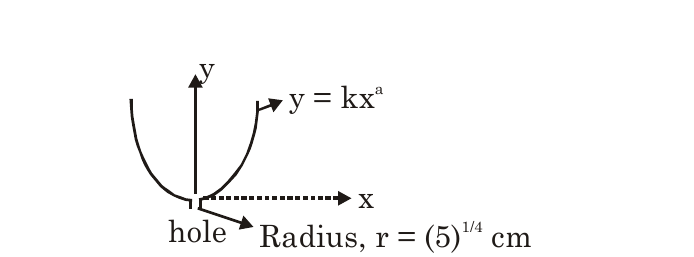
\includegraphics[width=0.55\linewidth]{Score-II - Test 01 (21 Mar 2021)-img/p2-phys-q1.png}
\end{center}

\begin{qoptions}
\opt{A}{If $k=1,\,a=4$, $t=12000$ sec.}
\opt{B}{If $k=1,\,a=2$, $t=500$ sec}
\opt{C}{If $k=4,\,a=2$, $t=125$ sec.}
\opt{D}{If $k=4,\,a=4$, $t=6000$ sec.}
\end{qoptions}

\textbf{2.} A uniform ring of radius $R$ lies on the x-y plane with its centre at origin. Its moment of inertia about z-axis is equal to its moment of inertia about an axis along the line $y=K_1x+K_2$.
\begin{qoptions}
\opt{A}{$K_1=1,\,K_2=+\dfrac{R}{\sqrt2}$}
\opt{B}{$K_1=1,\,K_2=-R$}
\opt{C}{$K_1=-1,\,K_2=+R$}
\opt{D}{$K_1=-1,\,K_2=-\dfrac{R}{\sqrt2}$}
\end{qoptions}

\textbf{3.} Three highly conducting concentric spherical shells (acting as black body) of radii $r_1$, $r_2$ and $r_3$ are kept in vacuum. The region between the shells is evacuated and they can exchange energy only by radiation. Inside the innermost shell there is a heater of constant power P. In steady state, ($\sigma=$ Stefan's constant)

\begin{center}
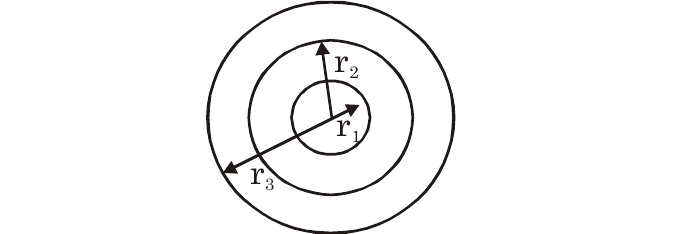
\includegraphics[width=0.45\linewidth]{Score-II - Test 01 (21 Mar 2021)-img/p2-phys-q3.png}
\end{center}

\begin{qoptions}
\opt{A}{Temperature of outermost shell is $\left(\dfrac{P}{4\pi\sigma r_3^2}\right)^{1/4}$}
\opt{B}{Temperature of middle shell is $\left(\dfrac{P}{4\pi\sigma}\right)^{1/4}\left(\dfrac1{r_3^2}+\dfrac1{r_2^2}\right)^{1/4}$}
\opt{C}{Temperature of innermost shell is $\left(\dfrac{P}{4\pi\sigma}\right)^{1/4}\left(\dfrac1{r_1^2}-\dfrac1{r_2^2}\right)^{1/4}$}
\opt{D}{If both outer and middle shell were removed, the temperature of innermost shell would decrease.}
\end{qoptions}

\textbf{4.} The system of two blocks is at rest as shown in the figure. A variable horizontal force is applied on the upper block. The coefficient of friction for both the contacts is $\mu$. Choose the correct option(s):

\begin{center}
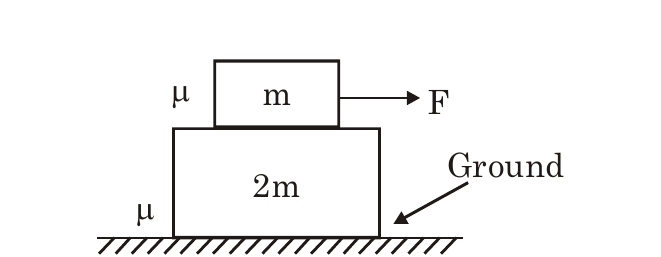
\includegraphics[width=0.5\linewidth]{Score-II - Test 01 (21 Mar 2021)-img/p2-phys-q4.png}
\end{center}

\begin{qoptions}
\opt{A}{When acceleration of the upper block is $2\mu g$, net force on the lower block by the ground is $mg\sqrt{9+\mu^2}$}
\opt{B}{When acceleration of the upper block is $2\mu g$, acceleration of the lower block is zero}
\opt{C}{Net horizontal force on the lower block is always zero.}
\opt{D}{Unless the upper block moves, no frictional force exists between the ground and the lower block.}
\end{qoptions}

\textbf{5.} In the diagram shown, a uniform magnetic field is present perpendicular to the plane of the paper. Both the rings are identical and have a constant resistance per unit length. The left ring has been kept fixed at its position and the right ring is slide uniformly on the left ring towards the right hand side. Which of the following statements is/are true?

\begin{center}
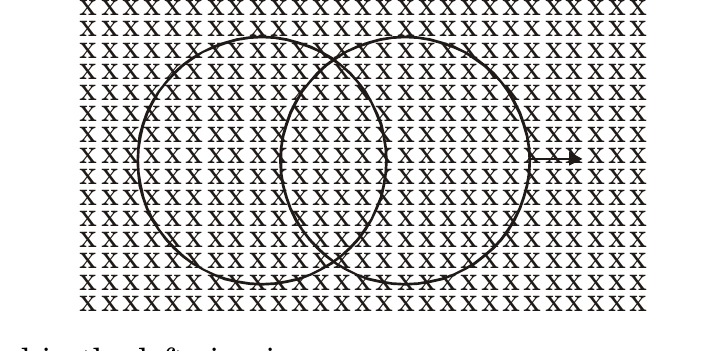
\includegraphics[width=0.6\linewidth]{Score-II - Test 01 (21 Mar 2021)-img/p2-phys-q5.png}
\end{center}

\begin{qoptions}
\opt{A}{The emf induced in the left ring is zero}
\opt{B}{The emf induced in both the rings is non-zero}
\opt{C}{The magnetic force acting on the right ring is zero}
\opt{D}{The magnetic force acting on both the rings is non-zero}
\end{qoptions}

\textbf{6.} In the circuit shown in figure, AB is a uniform wire of length $L=5$ m. It has a resistance of $2\,\Omega$/m. When AC $=2.0$ m, it was found that the galvanometer shows zero reading when switch S is placed in either of the two positions 1 or 2. Then,

\begin{center}
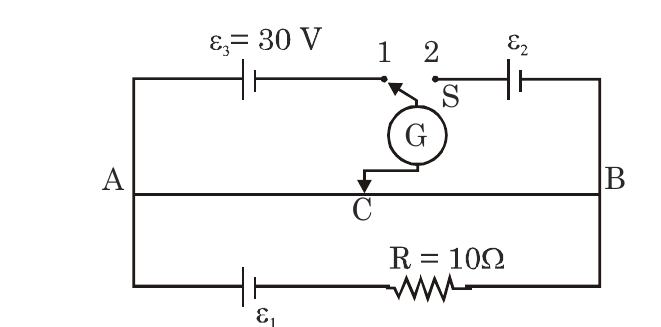
\includegraphics[width=0.6\linewidth]{Score-II - Test 01 (21 Mar 2021)-img/p2-phys-q6.png}
\end{center}

\begin{qoptions}
\opt{A}{$\varepsilon_1=150$V}
\opt{B}{$\varepsilon_1=600$V}
\opt{C}{$\varepsilon_2=60$V}
\opt{D}{$\varepsilon_2=45$V}
\end{qoptions}

\subsectionhdr{Section-I (ii): Matching Lists (single correct)}

\textbf{7.} Answer the following by appropriately matching the lists based on the information given in the list. $\dfrac{3}{25}$ moles of an ideal monatomic gas undergoes a process as shown in figure. $\Delta U$, Q and W represent the change in internal energy, amount of heat exchange and pressure-volume work respectively for the gas either for single process or for complete cycle. $\left(R=\dfrac{25}{3}\text{ SI unit}\right)$

\begin{center}
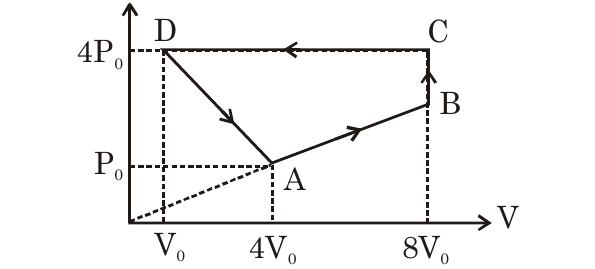
\includegraphics[width=0.55\linewidth]{Score-II - Test 01 (21 Mar 2021)-img/p2-phys-pv-graph.png}
\end{center}

\begin{center}
\begin{tabular}{@{}p{0.55\linewidth}p{0.35\linewidth}@{}}
\textbf{List-I} & \textbf{List-II} \\
(P) In process AB & (1) Q $=0$ or Q $=+$ve \\
(Q) In process DA & (2) $\Delta U=0$ or $\Delta U=-$ve \\
(R) In cyclic process ABCDA & (3) $\Delta U=+$ve \\
(S) In process CD & (4) W $=+$ve or W $=0$ \\
 & (5) W $=-$ve \\
\end{tabular}
\end{center}

Correctly match among the following is:
\begin{qoptions}
\opt{A}{P$\to$1,4; Q$\to$1,2,4; R$\to$2,5; S$\to$3,5}
\opt{B}{P$\to$1,3,4; Q$\to$1,2,4; R$\to$2,5; S$\to$2,5}
\opt{C}{P$\to$1,3,4; Q$\to$1,2,5; R$\to$2,5; S$\to$2,5}
\opt{D}{P$\to$1,3,4; Q$\to$1,2,4; R$\to$2,4; S$\to$2,5}
\end{qoptions}

\textbf{8.} Answer the following by appropriately matching the lists based on the information given in the list. $\dfrac{3}{25}$ moles of an ideal monatomic gas undergoes a process as shown in figure (same figure as Q.7). If temperature at point A is 100 K. $\left(R=\dfrac{25}{3}\text{ SI unit}\right)$

\begin{center}
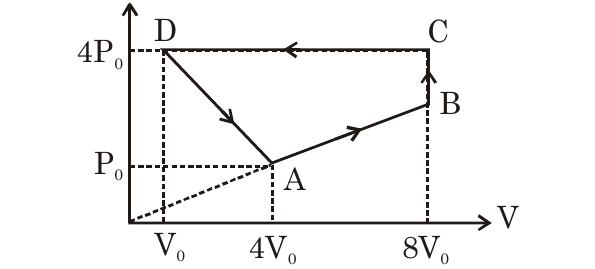
\includegraphics[width=0.55\linewidth]{Score-II - Test 01 (21 Mar 2021)-img/p2-phys-pv-graph.png}
\end{center}

\begin{center}
\begin{tabular}{@{}p{0.6\linewidth}p{0.3\linewidth}@{}}
\textbf{List-I} & \textbf{List-II} \\
(P) Work done in process AB & (1) 450 J \\
(Q) Change in internal energy in process AB & (2) 2100 J \\
(R) Work done in cyclic process ABCDA & (3) 150 J \\
(S) Change in internal energy in process CD & (4) 1050 J \\
 & (5) 362.5 J \\
\end{tabular}
\end{center}

Correctly match among the following is:
\begin{qoptions}
\opt{A}{P$\to$3; Q$\to$1; R$\to$5; S$\to$4}
\opt{B}{P$\to$3; Q$\to$2; R$\to$5; S$\to$4}
\opt{C}{P$\to$2; Q$\to$1; R$\to$5; S$\to$4}
\opt{D}{P$\to$3; Q$\to$1; R$\to$5; S$\to$2}
\end{qoptions}

\textbf{9.} Answer the following by appropriately matching the lists based on the information given in the list. If potential energy interaction between electron \& nucleus (infinite mass) is given by $U=-\dfrac{ke^2}{3r^3}$ (Bohr's theory is valid), where $n$ represents $n^{\text{th}}$ orbit, then:

\begin{center}
\begin{tabular}{@{}p{0.6\linewidth}p{0.25\linewidth}@{}}
\textbf{List-I} & \textbf{List-II} \\
(P) Electric current due to electron moving in a orbit & (1) $n^{-2}$ \\
(Q) Magnetic field due to electron at centre of atom & (2) $n^7$ \\
(R) Angular momentum of $n^{\text{th}}$ orbit & (3) $n^0$ \\
(S) Magnetic moment created due to revolving electron & (4) $n^5$ \\
 & (5) $n$ \\
\end{tabular}
\end{center}

\begin{qoptions}
\opt{A}{P$\to$4; Q$\to$2; R$\to$5; S$\to$5}
\opt{B}{P$\to$1; Q$\to$2; R$\to$5; S$\to$5}
\opt{C}{P$\to$4; Q$\to$2; R$\to$5; S$\to$1}
\opt{D}{P$\to$4; Q$\to$2; R$\to$1; S$\to$5}
\end{qoptions}

\textbf{10.} Answer the following by appropriately matching the lists based on the information given in the list. If potential energy interaction between electron \& nucleus (infinite mass) is given by $U=U_0\ln\left(\dfrac{r}{r_0}\right)$ (Bohr's theory is valid), where $n$ represents $n^{\text{th}}$ orbit, then:

\begin{center}
\begin{tabular}{@{}p{0.6\linewidth}p{0.25\linewidth}@{}}
\textbf{List-I} & \textbf{List-II} \\
(P) Electric current due to electron moving in a orbit & (1) $n^{-2}$ \\
(Q) Magnetic field due to electron at centre of atom & (2) $n^{-1}$ \\
(R) Angular momentum of $n^{\text{th}}$ orbit & (3) $n^0$ \\
(S) Magnetic moment created due to revolving electron & (4) $n^5$ \\
 & (5) $n$ \\
\end{tabular}
\end{center}

\begin{qoptions}
\opt{A}{P$\to$2; Q$\to$1; R$\to$2; S$\to$5}
\opt{B}{P$\to$2; Q$\to$1; R$\to$5; S$\to$5}
\opt{C}{P$\to$2; Q$\to$1; R$\to$4; S$\to$5}
\opt{D}{P$\to$3; Q$\to$1; R$\to$2; S$\to$5}
\end{qoptions}

\subsectionhdr{Section-II: Numerical Value}

\textbf{1.} Two point masses of mass $4m$ and $m$ respectively by a distance $d$ are revolving under mutual force of attraction. Ratio of their kinetic energy will be $\left(\dfrac{KE_{4m}}{KE_m}\right)$

\textbf{2.} A body is made of two rods AB and CD rigidly joined together to form a T shape. Two springs are attached to this body and the body is free to rotate in a vertical plane about a horizontal axis passing through C as shown in the figure. Then, the angular frequency (in rad/s) of small oscillation of this system is? Mass of each rod is $m=6$ kg and their lengths are $L=\dfrac{5}{52}$ m. Spring constant for each spring is $K=96$ N/m.

\begin{center}
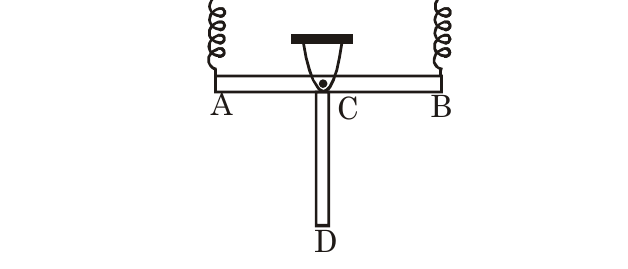
\includegraphics[width=0.55\linewidth]{Score-II - Test 01 (21 Mar 2021)-img/p2-phys-num-q2.png}
\end{center}

\textbf{3.} Inner surface of a cylindrical shell of length $\ell$ and of material of thermal conductivity $k$ is kept at constant temperature $T_1$ and the outer surface of the cylinder is kept at constant temperature $T_2$ such that ($T_1>T_2$) as shown in figure. Heat flows from inner surface to outer surface radially outward. Inner and outer radii of the shell are $R$ and $2R$ respectively. Due to lack of space this cylinder has to be replaced by a smaller cylinder of length $\dfrac{\ell}{2}$, inner and outer radii $\dfrac{R}{8}$ and $R$ respectively and thermal conductivity of material $nk$. If rate of radially outward heat flow remains same for same temperature of inner and outer surface i.e.\ $T_1$ and $T_2$, then find the value of $n$.

\begin{center}
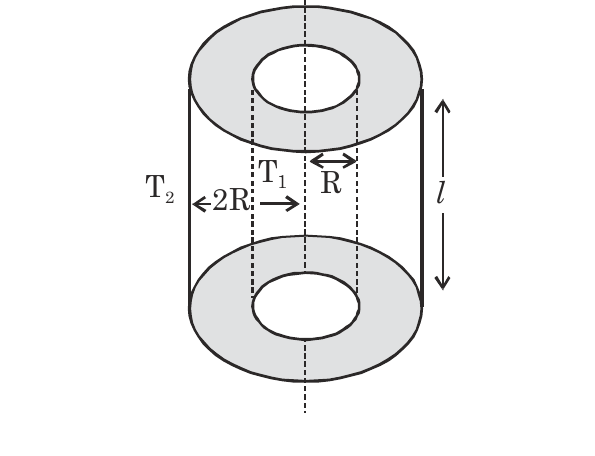
\includegraphics[width=0.5\linewidth]{Score-II - Test 01 (21 Mar 2021)-img/p2-phys-num-q3.png}
\end{center}

\textbf{4.} In the circuit shown, the reading of the Ammeter becomes four times of its initial value after the switch is closed. Each resistor has a resistance $=2\,\Omega$ and the ideal cell has e.m.f. $=10$ V. Then the ammeter has a resistance (in $\Omega$) equal to

\begin{center}
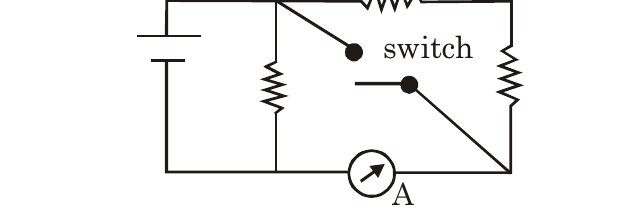
\includegraphics[width=0.5\linewidth]{Score-II - Test 01 (21 Mar 2021)-img/p2-phys-num-q4.png}
\end{center}

\textbf{5.} A long current carrying straight wire having current $I_1=10^4$ ampere is placed at the centre of another current carrying loop having current $I_2=10^4$ ampere. Straight wire is perpendicular to the plane of the loop as shown in the figure. The torque (in N-m) acting on the loop about its center is $10x$. Find the value of $x$. (Radius $R=1$m)

\begin{center}
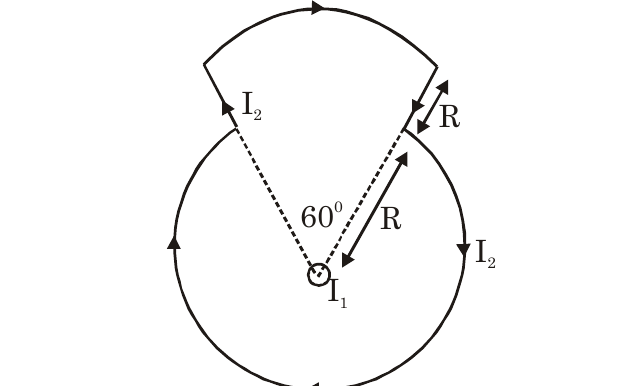
\includegraphics[width=0.55\linewidth]{Score-II - Test 01 (21 Mar 2021)-img/p2-phys-num-q5.png}
\end{center}

\textbf{6.} Consider a uniformly charged nonconducting cube of volume charge density $\rho$. Potential of one of vertex is $\dfrac{10}{3}$ volt, find the potential of centre of the cube (in volts).

\textbf{7.} If the length and breadth of a thin rectangular sheet are measured using a meter scale as 16.2 cm and 10.1 cm respectively, its surface area is $164\pm x$ cm$^2$. Then value of $x$ is.

\textbf{8.} Find the deviation of light ray (in degree)

\begin{center}
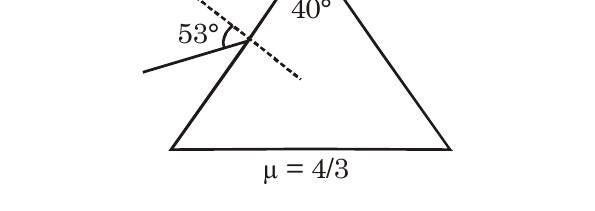
\includegraphics[width=0.45\linewidth]{Score-II - Test 01 (21 Mar 2021)-img/p2-phys-num-q8.png}
\end{center}

\sectionhdr{PART-2: CHEMISTRY}
\subsectionhdr{Section-I (i): Multiple Choice (one or more correct)}

\textbf{1.} Which phenomenon occurs when an electric field is applied to a colloidal solution and electrophoresis is prevented by some suitable means?
\begin{qoptions}
\opt{A}{Reverse osmosis takes place.}
\opt{B}{Electrosmosis takes place}
\opt{C}{Dispersion medium begins to move}
\opt{D}{Dispersion medium becomes stationary}
\end{qoptions}

\textbf{2.} Which of the following can have same set of quantum numbers?
\begin{qoptions}
\opt{A}{Unpaired electron of Cl and electron entered in Cl$^-$}
\opt{B}{Outermost electron of K and outermost electron of Cr}
\opt{C}{Paired electron in 2p-orbital of O and electron required to remove to form O$^+$ from O}
\opt{D}{Outermost electron of Mg and outermost electron of Ca}
\end{qoptions}

\textbf{3.} Correctly matched among the following is/are:

\begin{center}
\begin{tabular}{@{}p{4.6cm}p{2.9cm}@{}}
\toprule
\textbf{Column-I} & \textbf{Column-II} \\
\midrule
(A) 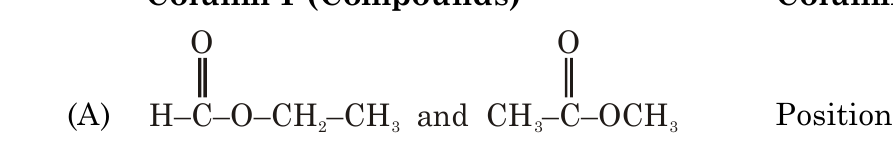
\includegraphics[width=4.3cm]{Score-II - Test 01 (21 Mar 2021)-img/p2-chem-q3-A.png} & Position Isomers \\[4pt]
(B) 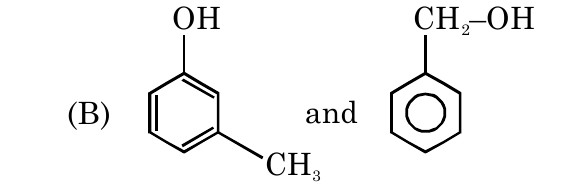
\includegraphics[width=4.3cm]{Score-II - Test 01 (21 Mar 2021)-img/p2-chem-q3-B.png} & Functional Isomers \\[4pt]
(C) 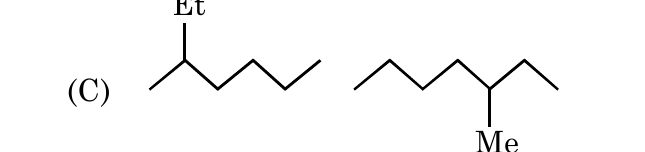
\includegraphics[width=4.3cm]{Score-II - Test 01 (21 Mar 2021)-img/p2-chem-q3-C.png} & Chain Isomers \\[4pt]
(D) 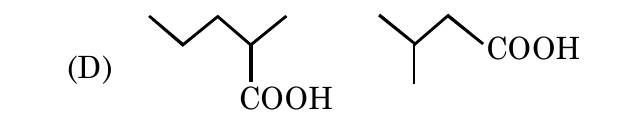
\includegraphics[width=4.3cm]{Score-II - Test 01 (21 Mar 2021)-img/p2-chem-q3-D.png} & Chain Isomers \\
\bottomrule
\end{tabular}
\end{center}

\textbf{4.} 80.0 gm salt of weak base and strong acid XY is dissolved in water and formed 2 litre of aqueous solution. The pH of the resultant solution was found to be 5 at 298 K. If XY forms CsCl type crystal having $r_{X^+}$ (radius of X$^+$) $=1.6$ \AA\ and $r_{Y^-}$ (radius of Y$^-$) $=1.864$ \AA\ then select correct statement(s). (Given: $K_b$(XOH) $=4\times10^{-5}$; $N_A=6\times10^{23}$, $\log 2=0.30$)
\begin{qoptions}
\opt{A}{Molar mass of salt is 100 g/mol}
\opt{B}{\% Degree of hydrolysis of salt is 0.25}
\opt{C}{Edge length of XY is 4 \AA}
\opt{D}{Density of solid salt XY is 5 in gm/cc}
\end{qoptions}

\textbf{5.} Which of the following statements are correct.
\begin{qoptions}
\opt{A}{In modern periodic table each block contains a number of columns equal to the number of electrons that can occupy that sub-shell.}
\opt{B}{The greatest increase in ionization enthalpy is experienced on removal of electron from core noble gas configuration.}
\opt{C}{The size of the isoelectronic species is affected by electron-electron interaction in the outer orbitals.}
\opt{D}{Anything that influences the valence electrons will affect the chemistry of the element and the valence shell is not affected by nuclear mass.}
\end{qoptions}

\textbf{6.} Correct option among the following is/are:
\begin{qoptions}
\opt{A}{Glycerol $+$ Oxalic acid $\xrightarrow{\text{(i) }100\text{--}110^{\circ}\text{, (ii) H}^+/\text{HOH}}$ Formic acid}
\opt{B}{Glycerol $+$ Oxalic acid $\xrightarrow{210^{\circ}}$ Allyl Alcohol}
\opt{C}{Glycol $+$ Oxalic acid $\xrightarrow{213^{\circ}\text{C}}$ Ethene}
\opt{D}{Glycerol $+$ Formic acid $\xrightarrow{260^{\circ}\text{C}}$ Allyl alcohol}
\end{qoptions}

\subsectionhdr{Section-I (ii): Matching Lists (single correct)}

\textbf{7.} Answer the following by appropriately matching the lists based on the information given in the list.

\begin{center}
\renewcommand{\arraystretch}{1.3}
\begin{tabular}{@{}p{4.0cm}p{3.7cm}@{}}
\textbf{List-I} & \textbf{List-II} \\
(P) 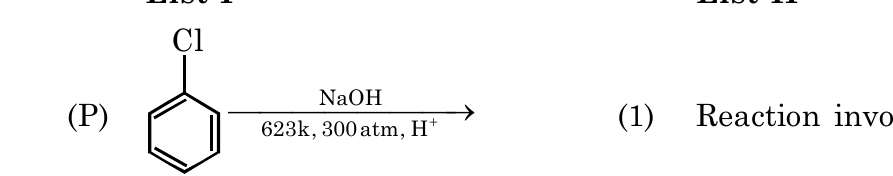
\includegraphics[width=3.7cm]{Score-II - Test 01 (21 Mar 2021)-img/p2-chem-q7-P.png} & (1) Reaction involve Meisenheimer Complex or anionic sigma complex \\[6pt]
(Q) 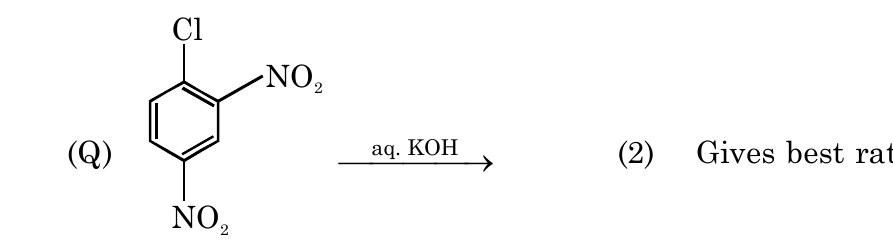
\includegraphics[width=3.7cm]{Score-II - Test 01 (21 Mar 2021)-img/p2-chem-q7-Q.png} & (2) Gives best rate of Ar S$_N$AE amongst all \\[6pt]
(R) 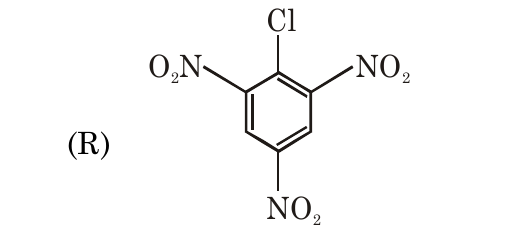
\includegraphics[width=3.0cm]{Score-II - Test 01 (21 Mar 2021)-img/p2-chem-q7-R.png} & (3) Benzyne intermediate is involved \\[6pt]
(S) 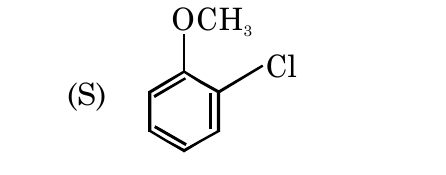
\includegraphics[width=2.4cm]{Score-II - Test 01 (21 Mar 2021)-img/p2-chem-q7-S.png} & (4) Raschig's Process \\
 & (5) $-$F instead of $-$Cl gives better rate of Ar S$_N$AE \\
\end{tabular}
\renewcommand{\arraystretch}{1.15}
\end{center}

Correctly match among the following is:
\begin{qoptions}
\opt{A}{P$\to$4; Q$\to$2,5; R$\to$1,3,5; S$\to$1}
\opt{B}{P$\to$3; Q$\to$1,5; R$\to$1,2,5; S$\to$3}
\opt{C}{P$\to$1; Q$\to$1,4; R$\to$1,5; S$\to$4}
\opt{D}{P$\to$2,3; Q$\to$1; R$\to$2,4,5; S$\to$1,3}
\end{qoptions}

\textbf{8.} Answer the following by appropriately matching the lists based on the information given in the list.

\begin{center}
\begin{tabular}{@{}p{0.25\linewidth}p{0.62\linewidth}@{}}
\textbf{List-I} & \textbf{List-II} \\
(P) N$_2^+$ \& NO & (1) Same bond order as that of B$_2$ \\
(Q) NF$^{-2}$ \& Cl$_2$ & (2) Same magnetic property and bond order as that of NO$^+$ \\
(R) CO \& CN$^-$ & (3) Same number of unpaired electron as that of S$_2^-$ \\
(S) C$_2$ \& CN$^+$ & (4) Same bond order but not same magnetic property as that of O$_2$ \\
 & (5) The bond order is less than that observed in CO$^+$ \\
 & (6) Similar magnetic property as that of O$_3$ \\
\end{tabular}
\end{center}

Correctly match among the following is:
\begin{qoptions}
\opt{A}{P$\to$3,4,5; Q$\to$1,4,6; R$\to$5; S$\to$4,5,6}
\opt{B}{P$\to$3,5,6; Q$\to$1,4,5; R$\to$2; S$\to$5,6}
\opt{C}{P$\to$3,5; Q$\to$1,5,6; R$\to$2,5; S$\to$4,5,6}
\opt{D}{P$\to$3,4,5; Q$\to$1,5; R$\to$2,4,5; S$\to$4,6}
\end{qoptions}

\textbf{9.} Answer the following by appropriately matching the lists based on the information given in the list.

\begin{center}
\begin{tabular}{@{}p{0.40\linewidth}p{0.52\linewidth}@{}}
\textbf{List-I} & \textbf{List-II} \\
(P) NH$_2$COONH$_4$(s) $\rightleftharpoons$ 2NH$_3$(g) $+$ CO$_2$(g); $\Delta H<0$ & (1) High pressure and low temperature will favour formation of products. \\
(Q) CaCO$_3$(s) $\rightleftharpoons$ CaO(s) $+$ CO$_2$(g); $\Delta H>0$ & (2) Increases in the amount of any of the product will definitely favour backward reaction. \\
(R) N$_2$(g) $+$ O$_2$(g) $\rightleftharpoons$ 2NO(g); $\Delta H>0$ & (3) Increase in temperature and doubling the volume of reaction vessel will cause the equilibrium to shift in similar direction. \\
(S) 2SO$_2$(g) $+$ O$_2$(g) $\rightleftharpoons$ 2SO$_3$(g); $\Delta H<0$ & (4) A decrease in temperature will cause decrease in the value of equilibrium constant. \\
 & (5) Increase in concentration of reactant the equilibrium is achieved will make the equilibrium shift towards product side \\
\end{tabular}
\end{center}

Correctly match among the following is:
\begin{qoptions}
\opt{A}{P$\to$3; Q$\to$3,5; R$\to$1,2,5; S$\to$3,4}
\opt{B}{P$\to$2; Q$\to$3,4; R$\to$2,4,5; S$\to$1,2,3,5}
\opt{C}{P$\to$2; Q$\to$4,5; R$\to$1,2,4; S$\to$1,3,5}
\opt{D}{P$\to$2; Q$\to$3,4,5; R$\to$1,4,5; S$\to$2,5}
\end{qoptions}

\subsectionhdr{Section-II: Numerical Value}

\textbf{1.} Find out Isoelectric value for Tyrosine.

\begin{center}
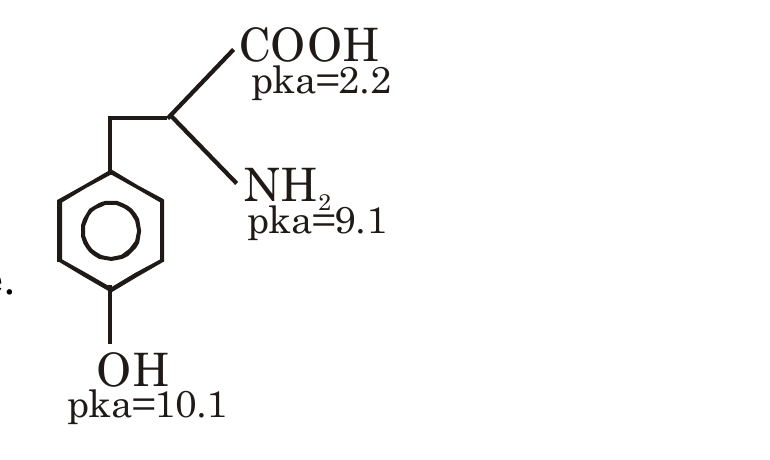
\includegraphics[width=0.55\linewidth]{Score-II - Test 01 (21 Mar 2021)-img/p2-chem-num-q1-tyrosine.png}
\end{center}

\textbf{2.} Among the following complexes, how many have spin only magnetic moment of 2.83 B.M.\\
$[\text{Ni(CO)}_4]$; $[\text{Ni(NH}_3)_6]^{+2}$; $[\text{NiCl}_2(\text{PPh}_3)_2]$; $[\text{NiCl}_4]^{-2}$; $[\text{NiF}_6]^{-2}$; $[\text{Ni(H}_2\text{O})_6]^{+2}$; $[\text{Ni(en)}_3]^{+2}$; $[\text{NiF}_6]^{-4}$; $[\text{Ni(CN)}_4]^{-2}$; $[\text{PdCl}_4]^{-2}$.

\textbf{3.} The graph of compressibility factor (Z) vs P for one mode of a real gas is plotted at constant temperature 273 K. If the slope of graph at very high pressure $\left(\dfrac{dZ}{dp}\right)$ is $\dfrac{1}{10}$ atm$^{-1}$, the volume of one molecule of real gas in cm$^3$ is $x \times 10^{-22}$. Find `x'. [Take $N_A = 6 \times 10^{23}$].

\textbf{4.} (a) Oxidation state of Zr in the compound formed by it in Van arkel process is $k$\\
(b) Bond order of gas used in Monds process is $l$\\
(c) Number of ions formed on dissolution of a complex formed after reduction in Macarthur forrest process of extracting silver is $m$.\\
Report your answer as $(k \times l \times m)$

\textbf{5.} Number of compounds which can be oxidised by Tollen's regent.

\begin{center}
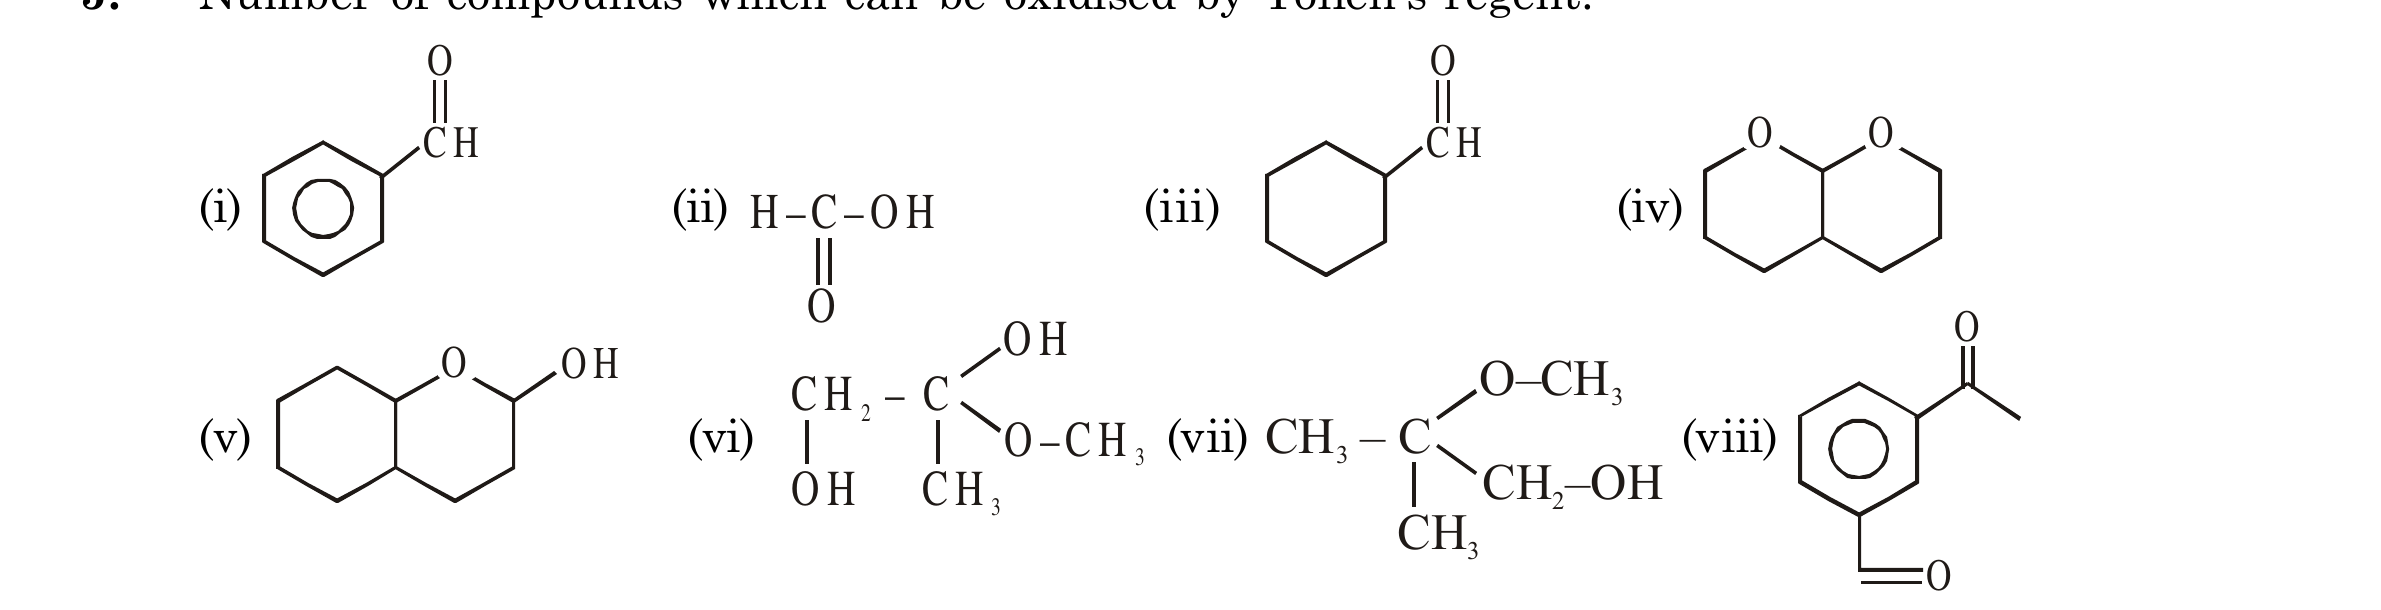
\includegraphics[width=0.95\linewidth]{Score-II - Test 01 (21 Mar 2021)-img/p2-chem-num-q5-structs.png}
\end{center}

\textbf{6.} Solution of HNO$_3$ in pure H$_2$SO$_4$ can be used for nitration of benzene. One such solution was made by adding 63 gm HNO$_3$ in 9800 gm H$_2$SO$_4$. What should be the approx. molality of all particles in this solution if 30\% HNO$_3$ is dissociated?

\textbf{7.} Amongst the following, the total number of compounds soluble in concentrated NH$_3$ solution is
\begin{center}
\begin{tabular}{@{}ll@{}}
(A) Ag$_2$CrO$_4$ & (B) Cu(OH)$_2\cdot$CuSO$_4$ \\
(C) PbSO$_3$ & (D) Al(OH)$_3$ \\
(E) Ni(OH)$_2$ & (F) Zn$_3$(PO$_4$)$_2$ \\
(G) BaSO$_4$ & (H) Bi(OH)$_2$NO$_3$ \\
(I) Mn(OH)$_2$ & \\
\end{tabular}
\end{center}

\textbf{8.} How many compounds gives chloroform with Cl$_2$, NaOH?

\begin{center}
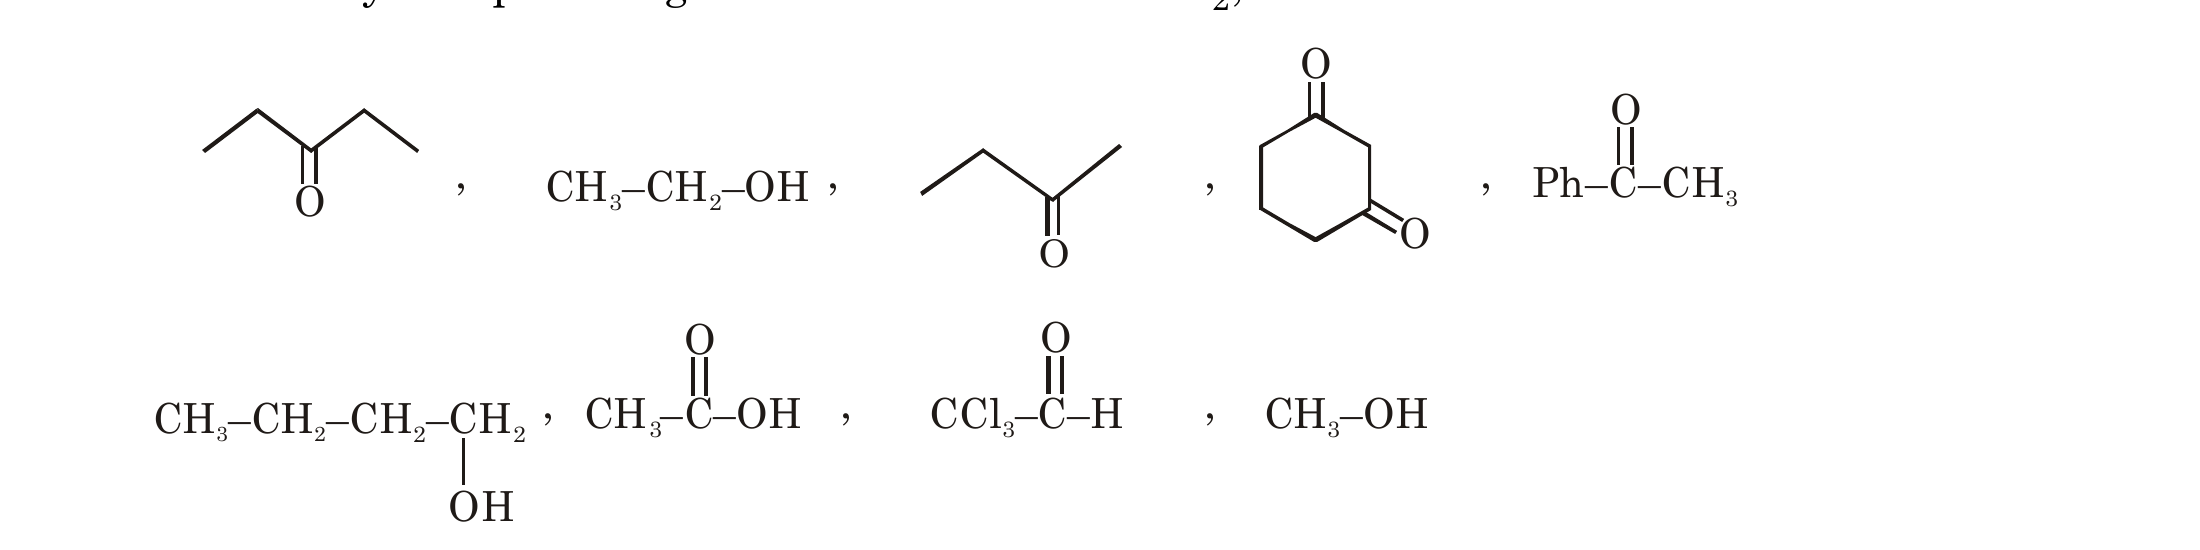
\includegraphics[width=0.95\linewidth]{Score-II - Test 01 (21 Mar 2021)-img/p2-chem-num-q8-structs.png}
\end{center}

\sectionhdr{PART-3: MATHEMATICS}
\subsectionhdr{Section-I (i): Multiple Choice (one or more correct)}

\textbf{1.} Let E-ABCD be a pyramid on square base ABCD where A is the origin and B and D are lying on positive x-axis and y-axis respectively. If E is $(0,2,3)$ and $\overrightarrow{DE}\cdot(\hat{i}+\hat{j})=\vec{0}$, then
\begin{qoptions}
\opt{A}{image of the point D in the plane ABE is $\left(0,\dfrac{-10}{13},\dfrac{24}{13}\right)$}
\opt{B}{image of the point D in the plane ABE is $\left(0,\dfrac{-6}{13},\dfrac{30}{13}\right)$}
\opt{C}{volume of the tetrahedron ABDE is 2 cubic units.}
\opt{D}{perpendicular distance of the point D from the plane ABE is $\dfrac{9}{\sqrt{13}}$}
\end{qoptions}

\textbf{2.} Let $z_1,z_2,z_3\in\mathbb{C}$ and satisfying $z_1\bar z_1+(2+3i)\bar z_1+(2-3i)z_1=3=z_2\bar z_2+(2+3i)\bar z_2+(2-3i)z_2$ and $z_3=4+6i$. If $\arg(z_3-z_1)=\arg(z_3-z_2)$ then
\begin{qoptions}
\opt{A}{$|z_3-z_1|\,|z_3-z_2|=101$}
\opt{B}{$|z_3-z_1|\,|z_3-z_2|=117$}
\opt{C}{If $|z_1-z_2|$ is maximum then $|z_1z_2|=3$}
\opt{D}{If $|z_1-z_2|$ is maximum then $|z_1|+|z_2|=8$}
\end{qoptions}

\textbf{3.} Let $A$ be a non singular square matrix of order 3 such that $\text{Tr.}(A^{-1})=3$ and $\det(A^{-1})=\dfrac{1}{5}$. If $(A^{-1}BA)=2(\text{adj }A)$ then
\begin{qoptions}
\opt{A}{$\det(B)=5000$}
\opt{B}{$\det(B)=200$}
\opt{C}{$\text{Tr.}(B)=30$}
\opt{D}{$\text{Tr.}(B)=15$}
\end{qoptions}
[Note: Tr.(P) and adj P denote trace of square matrix P and adjoint matrix of square matrix P respectively.]

\textbf{4.} Two tangents $2x+y=2$ and $x-2y=3$ to a parabola touching it at $A(2,-2)$ and $B(5,1)$ respectively. If focus of parabola is $S(\alpha,\beta)$ and latus rectum length is $L$ then $(\alpha,\beta\in\mathbb{R})$
\begin{qoptions}
\opt{A}{$\alpha-\beta=3$}
\opt{B}{$\alpha-\beta=4$}
\opt{C}{$L=\dfrac{27\sqrt3}{25}$}
\opt{D}{$L=\dfrac{27\sqrt2}{25}$}
\end{qoptions}

\textbf{5.} If $I_1=\dfrac{\displaystyle\int_0^{\pi/4}\left(x-\dfrac{\pi}{4}\right)^{50}\cdot\sec^2x\,dx}{\displaystyle\int_0^{\pi/4}\left(x-\dfrac{\pi}{4}\right)^{49}\cdot\tan x\,dx}$

$I_2=\dfrac{1}{100}\displaystyle\int_0^{\pi/4}\left(x-\dfrac{\pi}{4}\right)^{100}\cdot\sec^2x\,dx-\displaystyle\int_0^{\pi/4}x^{99}\cdot\left(\dfrac{1-\tan x}{1+\tan x}\right)dx$ then
\begin{qoptions}
\opt{A}{$I_1<I_2$}
\opt{B}{$I_1>I_2$}
\opt{C}{$I_1\cdot I_2\ge0$}
\opt{D}{$I_1\cdot I_2<0$}
\end{qoptions}

\textbf{6.} In a triangle ABC, which of the following is/are true?
\begin{qoptions}
\opt{A}{$\dfrac{\cos A}{a}=\dfrac{\cos B}{b}=\dfrac{\cos C}{c}$}
\opt{B}{$\dfrac{\cos A}{a}+\dfrac{\cos B}{b}+\dfrac{\cos C}{c}=\dfrac{a^2+b^2+c^2}{2abc}$}
\opt{C}{$\dfrac{1}{r_1}+\dfrac{1}{r_2}+\dfrac{1}{r_3}=\dfrac{1}{r}$}
\opt{D}{$\dfrac{\sin2A}{a^2}=\dfrac{\sin2B}{b^2}=\dfrac{\sin2C}{c^2}$}
\end{qoptions}
(where symbols have their usual meaning in a triangle)

\subsectionhdr{Section-I (ii): Matching Lists (single correct)}

\textbf{7.} Answer the following by appropriately matching the lists based on the information given in the list.

Let $g(x)=\begin{cases}\dfrac{\pi}{2}-2\tan^{-1}(f(x)), & f(x)\in(-1,1)\\[4pt] -\dfrac{\pi}{2}-2\tan^{-1}(f(x)), & f(x)\in(-\infty,-1)\\[4pt] \dfrac{3\pi}{2}-2\tan^{-1}(f(x)), & f(x)\in(1,\infty)\end{cases}$, where $f(x)=\begin{cases}x+1, & x\le0\\ 1-x^2, & 0<x<2\\ x-5, & x\ge2\end{cases}$

\begin{center}
\renewcommand{\arraystretch}{1.25}
\begin{tabular}{@{}p{5.4cm}p{2.2cm}@{}}
\textbf{List-I} & \textbf{List-II} \\
(P) Values of `x' for which derivative of $g(x)$ w.r.t. $f(x)$ is $-\dfrac{1}{13}$ is/are & (1) $-6$ \\[4pt]
(Q) Values of `x' for which $f(x)$ has local maximum or local minimum & (2) 1 \\[4pt]
(R) Values of `k' for which $f(x)+k=0$ has 2 positive and one negative root is/are & (3) 2 \\[4pt]
(S) Values of `x' for which $g'(x)<0$ is/are & (4) 10 \\
\end{tabular}
\renewcommand{\arraystretch}{1.15}
\end{center}

Correctly match among the following is:
\begin{qoptions}
\opt{A}{P$\to$1,4; Q$\to$3; R$\to$2,3; S$\to$1,4}
\opt{B}{P$\to$1,3; Q$\to$4; R$\to$2,3; S$\to$1,4}
\opt{C}{P$\to$1,3; Q$\to$3; R$\to$2,4; S$\to$1,3}
\opt{D}{P$\to$1,4; Q$\to$4; R$\to$2,1; S$\to$1,3}
\end{qoptions}

\textbf{8.} Answer the following by appropriately matching the lists based on the information given in the list.

\begin{center}
\renewcommand{\arraystretch}{1.25}
\begin{tabular}{@{}p{5.6cm}p{1.6cm}@{}}
\textbf{List-I} & \textbf{List-II} \\
(P) The curve $y=f(x)$ satisfies $\dfrac{d^2y}{dx^2}=6x-4$ and $f(x)$ has a local minimum value 5 when $x=1$. Then $f(0)$ is equal to & (1) 1 \\[6pt]
(Q) The tangent to $y=ax^2+bx+\dfrac{7}{2}$ at $(1,2)$ is parallel to the normal at $(-2,2)$ on the curve $y=x^2+6x+8$. Then the value of $\dfrac{a}{2}-b$ is & (2) 2 \\[6pt]
(R) Let A be the point where the curve $5a^2x^3+10ax^2+x+2y-4=0$ ($a\in\mathbb{R}, a\ne0$) meets the y-axis, then the equation of tangent to the curve at the point where the normal at A meets the curve again is $y=ax+b$, then the value of $a+b$ is & (3) 3 \\[6pt]
(S) If $f(x)=-\dfrac{px}{e^x}+\dfrac{x^2}{2}$ is a decreasing function for every $x\le0$. Then the least value of $p^2$ is & (4) 4 \\[2pt]
 & (5) 5 \\
\end{tabular}
\renewcommand{\arraystretch}{1.15}
\end{center}

Correctly match among the following is:
\begin{qoptions}
\opt{A}{P$\to$5, Q$\to$3, R$\to$4, S$\to$2}
\opt{B}{P$\to$5, Q$\to$2, R$\to$4, S$\to$1}
\opt{C}{P$\to$5, Q$\to$3, R$\to$4, S$\to$1}
\opt{D}{P$\to$4, Q$\to$3, R$\to$2, S$\to$2}
\end{qoptions}

\textbf{9.} Answer the following by appropriately matching the lists based on the information given in the list.

\begin{center}
\renewcommand{\arraystretch}{1.25}
\begin{tabular}{@{}p{5.6cm}p{1.6cm}@{}}
\textbf{List-I} & \textbf{List-II} \\
(P) If $f(x)=\text{sgn}(\sin^2x-\sin x-1)$ has exactly 4 points of discontinuity for $x\in(0,n\pi)$, $n\in\mathbb{N}$ then $n$ can be & (1) 0 \\[6pt]
(Q) Let $f(x)=x^2-x+k-2$ and $g(x)=x^2-x+1$. If the complete set of values of $k$ for which $y=\left[\dfrac{f(x)}{g(x)}\right]$ (where $[\cdot]$ denotes greatest integer function) is continuous $\forall x\in\mathbb{R}$ is $[a,b)$ then $\left(b-\dfrac{5a}{4}\right)$ equals & (2) 4 \\[10pt]
(R) Let $f(x)=\begin{cases}\cos^{-1}x, & \tfrac12\le x\le1\\ \tfrac{2}{3}x+\tfrac{\pi}{3}-\tfrac13, & x<\tfrac12\end{cases}$. Then the number of real points in the domain of $f(x)$ where it is non-differentiable is & (3) 5 \\[10pt]
(S) Number of points where $f(x)=\begin{cases}\max\!\big(|x^2-x-2|,\,x^2-3x\big), & x\ge0\\ \max\!\big(\ln(-x),\,e^x\big), & x<0\end{cases}$ is non-differentiable is & (4) 3 \\
 & (5) 2 \\
\end{tabular}
\renewcommand{\arraystretch}{1.15}
\end{center}

Correctly match among the following is:
\begin{qoptions}
\opt{A}{P$\to$2,3; Q$\to$1; R$\to$3; S$\to$4}
\opt{B}{P$\to$2,3; Q$\to$1; R$\to$2; S$\to$4}
\opt{C}{P$\to$2,4; Q$\to$5; R$\to$2; S$\to$5}
\opt{D}{P$\to$2,4; Q$\to$5; R$\to$3; S$\to$5}
\end{qoptions}

\textbf{10.} Answer the following by appropriately matching the lists based on the information given in the list.

Let $f(x)=\displaystyle\lim_{t\to\infty}\dfrac{(a+\sin\pi x)^t-1}{(a+\sin\pi x)^t+1}$, $x\in(0,6)$, then

\begin{center}
\renewcommand{\arraystretch}{1.25}
\begin{tabular}{@{}p{2.6cm}p{4.6cm}@{}}
\textbf{List-I} & \textbf{List-II} \\
(P) If $a=1$, then & (1) $f(x)$ has no point of discontinuity \\[4pt]
(Q) If $a=3$, then & (2) $f(x)$ has 5 points of discontinuity \\[4pt]
(R) If $a=0.5$, then & (3) $f(x)$ has infinite points of discontinuity \\[4pt]
(S) If $a=0$, then & (4) $f(x)$ has 6 points of discontinuity \\[4pt]
 & (5) $f(x)$ has 3 points of discontinuity \\
\end{tabular}
\renewcommand{\arraystretch}{1.15}
\end{center}

Correctly match among the following is:
\begin{qoptions}
\opt{A}{P$\to$2; Q$\to$1; R$\to$4; S$\to$4}
\opt{B}{P$\to$4; Q$\to$1; R$\to$4; S$\to$3}
\opt{C}{P$\to$5; Q$\to$4; R$\to$5; S$\to$2}
\opt{D}{P$\to$2; Q$\to$4; R$\to$5; S$\to$4}
\end{qoptions}

\subsectionhdr{Section-II: Numerical Value}

\textbf{1.} $\hat n$ is a vector perpendicular to the plane containing the points whose position vectors are $\vec a,\vec b$ and $\vec r$, satisfying $\big[\vec r-\vec a\ \ \vec b-\vec a\ \ \hat n\big]=\lambda\,\vec r\times(\vec b-\vec a)-\vec a\times\vec b$ then the value of $\lambda$ is

\textbf{2.} Consider the two circles $C_1: x^2+y^2+4x+4y-1=0$, $C_2: x^2+y^2+6x+2y-7=0$ and the two lines $L_1: x+2y+3=0$, $L_2: 2x+3y+\lambda=0$. If $L_1$ intersects $C_1$ at $A$ and $B$ and $L_2$ intersects $C_2$ at $C$ and $D$, the value of $\lambda$ so that $A,B,C,D$ are concyclic is

\textbf{3.} Consider the differential equation $\sin y\,dy=2\cos x\cos y\,dx-\sin^2x\cos x\,dx$ where $y|_{x=0}=0$. If the solution of the differential equation is expressed in the form $\cos y=A\sin^2x+B\sin x+C+De^{-2\sin x}$ where $A,B,C,D$ are constants. Find $(A+B+C+D)$.

\textbf{4.} A box contains $n$ coins of which atleast one is biased. Let $E_k$ denote the event that exactly $k$ out of the $n$ coins are biased. Also let $P(E_k)$ be directly proportional to $k(k+1)$ for $1\le k\le n$. If a coin selected at random is found to be biased, then the probability that it is the only biased coin in the box is $F(n)$. Find $\displaystyle\lim_{k\to\infty}\sum_{r=1}^{k}F(r)\cdot(3r+1)$.

\textbf{5.} Let $a_1,a_2,a_3,\ldots,a_9$ be in H.P. where $a_4=5$ and $a_5=4$.

If $D=\begin{vmatrix}a_1 & a_2 & a_3\\ 5 & 4 & a_6\\ a_7 & a_8 & a_9\end{vmatrix}$ and $A=\begin{bmatrix}1 & 1/2 & 1/3\\ 1/4 & 1/5 & 1/6\\ 1/7 & 1/8 & 1/9\end{bmatrix}$ then $\dfrac{D}{1000|A|}$ is equal to

\textbf{6.} Let matrix $A=\begin{vmatrix}x & y & -z\\ 1 & 2 & 3\\ 1 & 1 & 2\end{vmatrix}$, where $x,y,z\in\mathbb{N}$. If $|\text{adj}(\text{adj}(\text{adj}(\text{adj}\,A)))|=4^8\cdot5^{16}$, then the value of $(x+y+z)$ equals

\textbf{7.} If $a_1,a_2,a_3,\ldots,a_n$ be in A.P. Let $(1+\sin2\theta)$ is the A.M. of $a_1,a_n$. Let $(1-\tan\theta)$ is the A.M. of $\dfrac{1}{a_1a_n},\dfrac{1}{a_2a_{n-1}},\ldots,\dfrac{1}{a_na_1}$. Let $(1+\tan\theta)$ is the A.M. of $\dfrac{1}{a_1},\dfrac{1}{a_2},\dfrac{1}{a_3}\ldots\dfrac{1}{a_n}$. Then the sum of values of $\theta\in(0,2\pi]$ is $k\pi$. Find $k$.

\textbf{8.} Let $t_{100}=\displaystyle\sum_{r=0}^{100}\dfrac{1}{\left({}^{100}C_r\right)^5}$ and $S_{100}=\displaystyle\sum_{r=0}^{100}\dfrac{r}{\left({}^{100}C_r\right)^5}$, then the value of $\dfrac{S_{100}}{5t_{100}}$ equals

\end{document}
